\section{Předzpracování a rámce}

Před tím než začneme pracovat se signálem je hlavní tento signál normalizovat, aby jsme dostali nějaké rozumné hodnoty s kterými pracovat.
Tato část je hlavně důležitá pokud chceme porovávat signály mezi sebou. Další důvod normalizace je pro využité některých algoritmů které neumí pracovat s daty co nejsou normalizované.

\begin{figure}[H] 
	\centering
	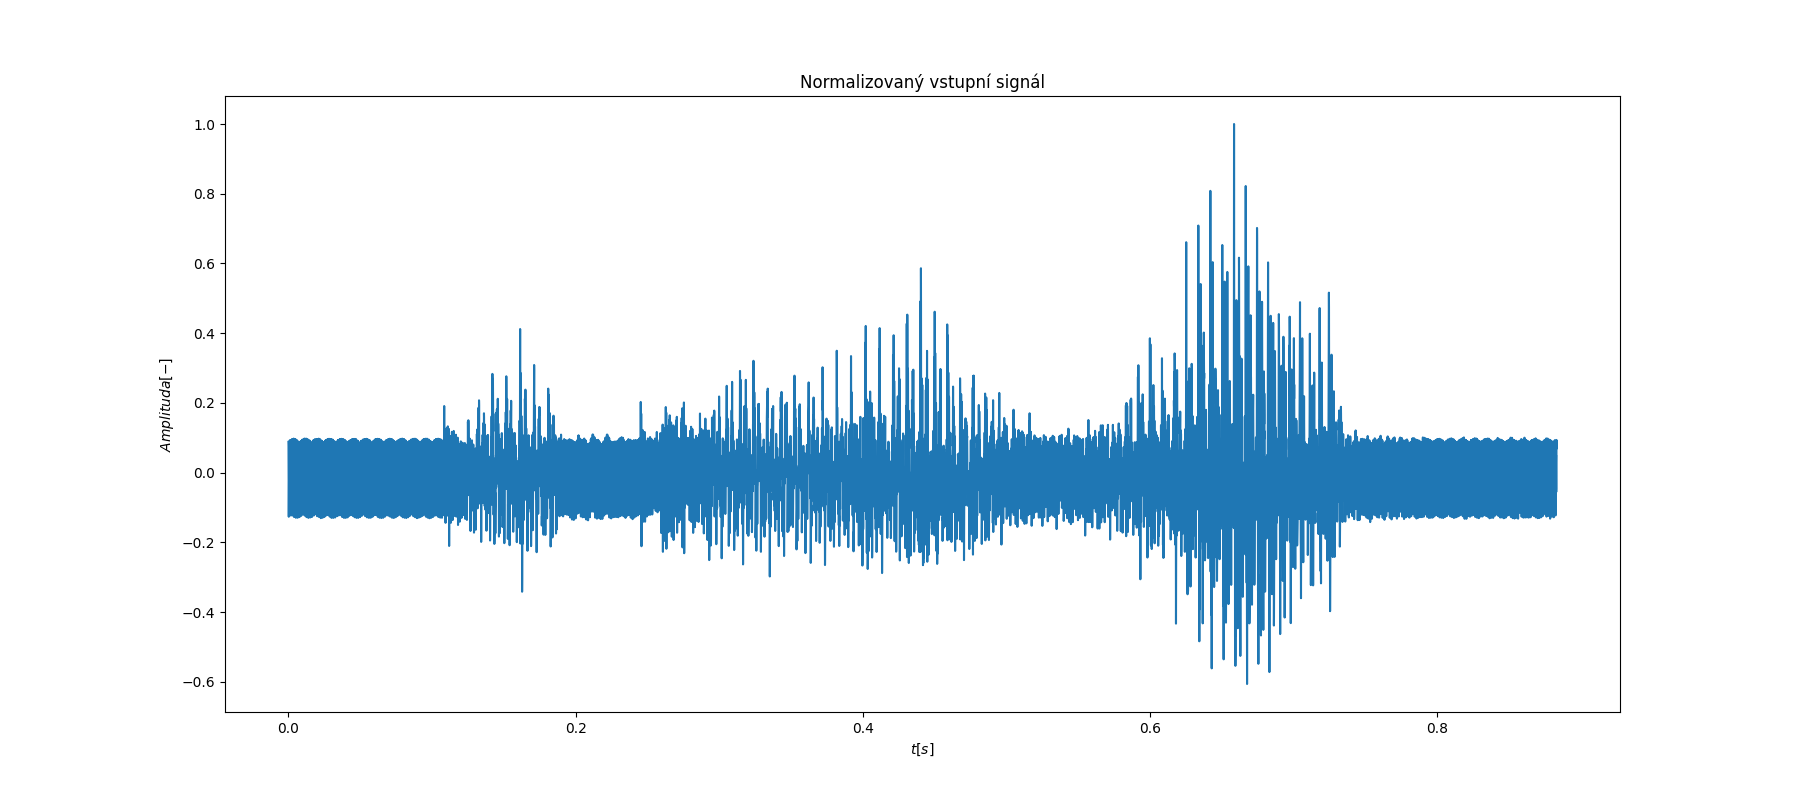
\includegraphics[scale=0.35,keepaspectratio]{Figure_3}
	\caption{Normalizovaný a vycentrovaný vstupní signál}
\end{figure}

\begin{figure}[H] 
	\centering
	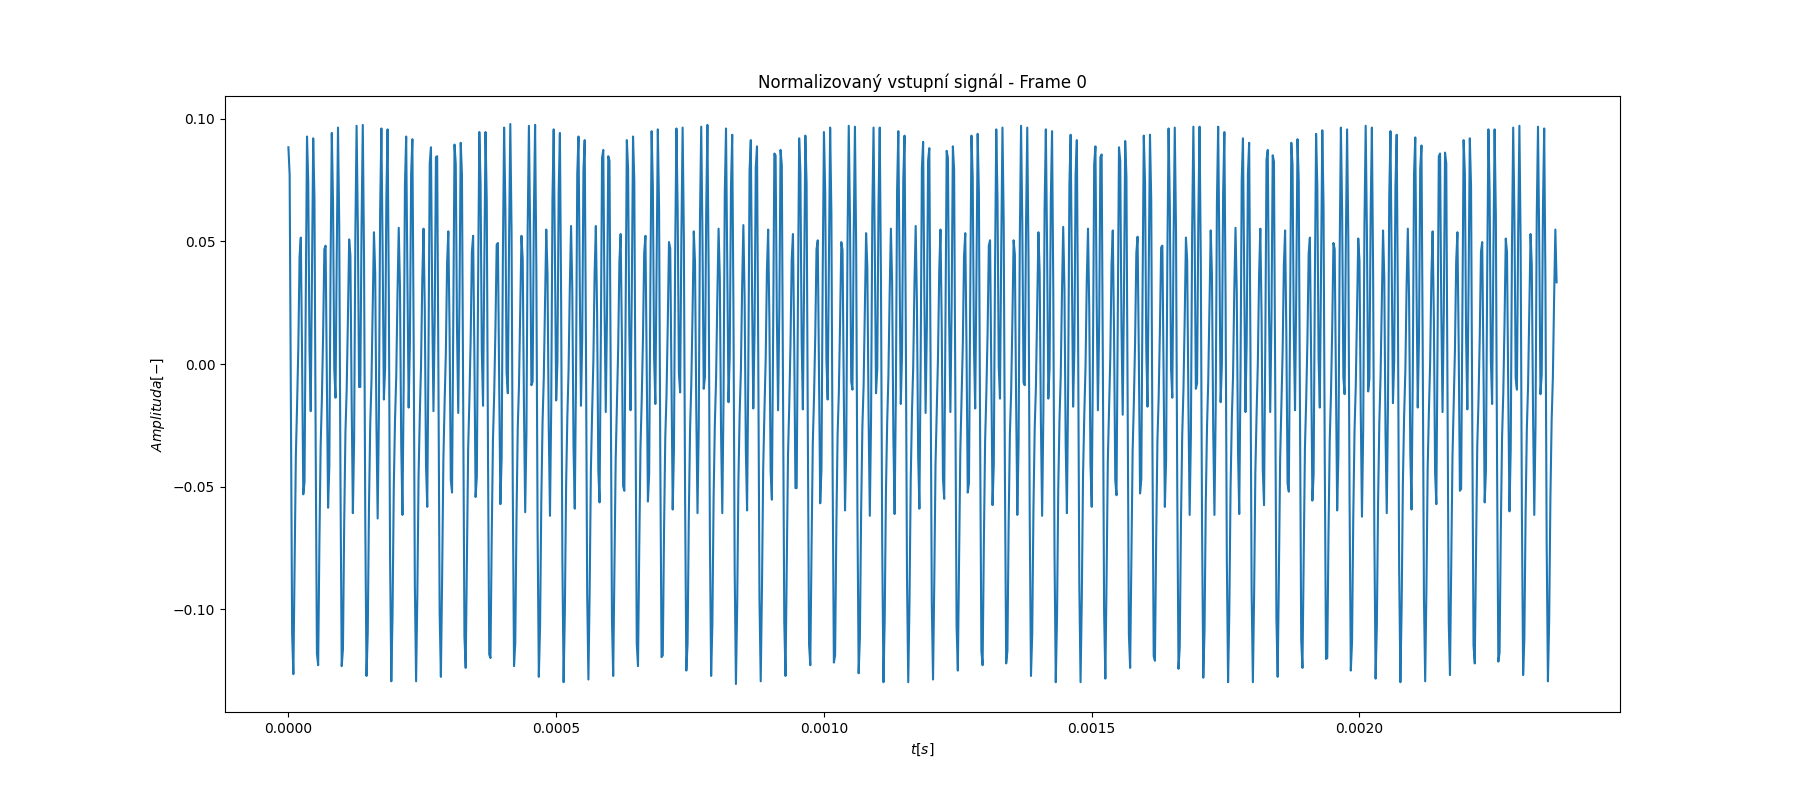
\includegraphics[scale=0.35,keepaspectratio]{Figure_2}
	\caption{Vycentrovaný a normalizovaný rámec \#0}
\end{figure}